%%%%%%%%%%%%%%%%%%%%%%%%%%%%%%%%%%%%%%%%%
% "ModernCV" CV and Cover Letter
% LaTeX Template
% Version 1.1 (9/12/12)
%
% This template has been downloaded from:
% http://www.LaTeXTemplates.com
%
% Original author:
% Xavier Danaux (xdanaux@gmail.com)
%
% License:
% CC BY-NC-SA 3.0 (http://creativecommons.org/licenses/by-nc-sa/3.0/)
%
% Important note:
% This template requires the moderncv.cls and .sty files to be in the same
% directory as this .tex file. These files provide the resume style and themes
% used for structuring the document.
%
%%%%%%%%%%%%%%%%%%%%%%%%%%%%%%%%%%%%%%%%%

%----------------------------------------------------------------------------------------
%	PACKAGES AND OTHER DOCUMENT CONFIGURATIONS
%----------------------------------------------------------------------------------------

\documentclass[11pt,a4paper,sans]{moderncv} % Font sizes: 10, 11, or 12; paper sizes: a4paper, letterpaper, a5paper, legalpaper, executivepaper or landscape; font families: sans or roman

\usepackage[latin1]{inputenc}
\usepackage[english,french]{babel}
\usepackage[T1]{fontenc}
\usepackage{wrapfig}

\moderncvstyle{classic} % CV theme - options include: 'casual' (default), 'classic', 'oldstyle' and 'banking'
\moderncvcolor{blue} % CV color - options include: 'blue' (default), 'orange', 'green', 'red', 'purple', 'grey' and 'black'

\usepackage[height=0.9\paperheight, width=1.37\linewidth]{geometry} % Reduce document margins
%\setlength{\hintscolumnwidth}{3cm} % Uncomment to change the width of the dates column
%\setlength{\makecvtitlenamewidth}{10cm} % For the 'classic' style, uncomment to adjust the width of the space allocated to your name

\usepackage{color}

\newenvironment{myfont}{\fontfamily{ptm}\fontsize{13pt}{16pt}\selectfont}{\par}

%----------------------------------------------------------------------------------------
%	NAME AND CONTACT INFORMATION SECTION
%----------------------------------------------------------------------------------------

\firstname{\Huge \qquad Fran\c{c}ois} % Your first name
\familyname{\Huge THIERRY} % Your last name

% All information in this block is optional, comment out any lines you don't need
\title{\qquad\quad MEng - MSc - PhD}
\address{1 impasse Antoine Watteau\\}{45650 Saint Jean le Blanc, France}
\mobile{+33 (0)6 75 49 39 28}
%\phone{(000) 111 1112}
%\fax{(000) 111 1113}
\email{francois.thierry90@gmail.com}
\homepage{francois-thierry.github.io}{} % The first argument is the url for the clickable link, the second argument is the url displayed in the template - this allows special characters to be displayed such as the tilde in this example
\extrainfo{26 Years Old, Single}
% \photo[45pt][0pt]{photo.jpg} % The first bracket is the picture height, the second is the thickness of the frame around the picture (0pt for no frame)

%----------------------------------------------------------------------------------------
%   START OF THE DOCUMENT
%----------------------------------------------------------------------------------------
\begin{document}

~\

\begin{wrapfigure}{l}{25pt}
  \centering
  \vspace{-2.6cm}
  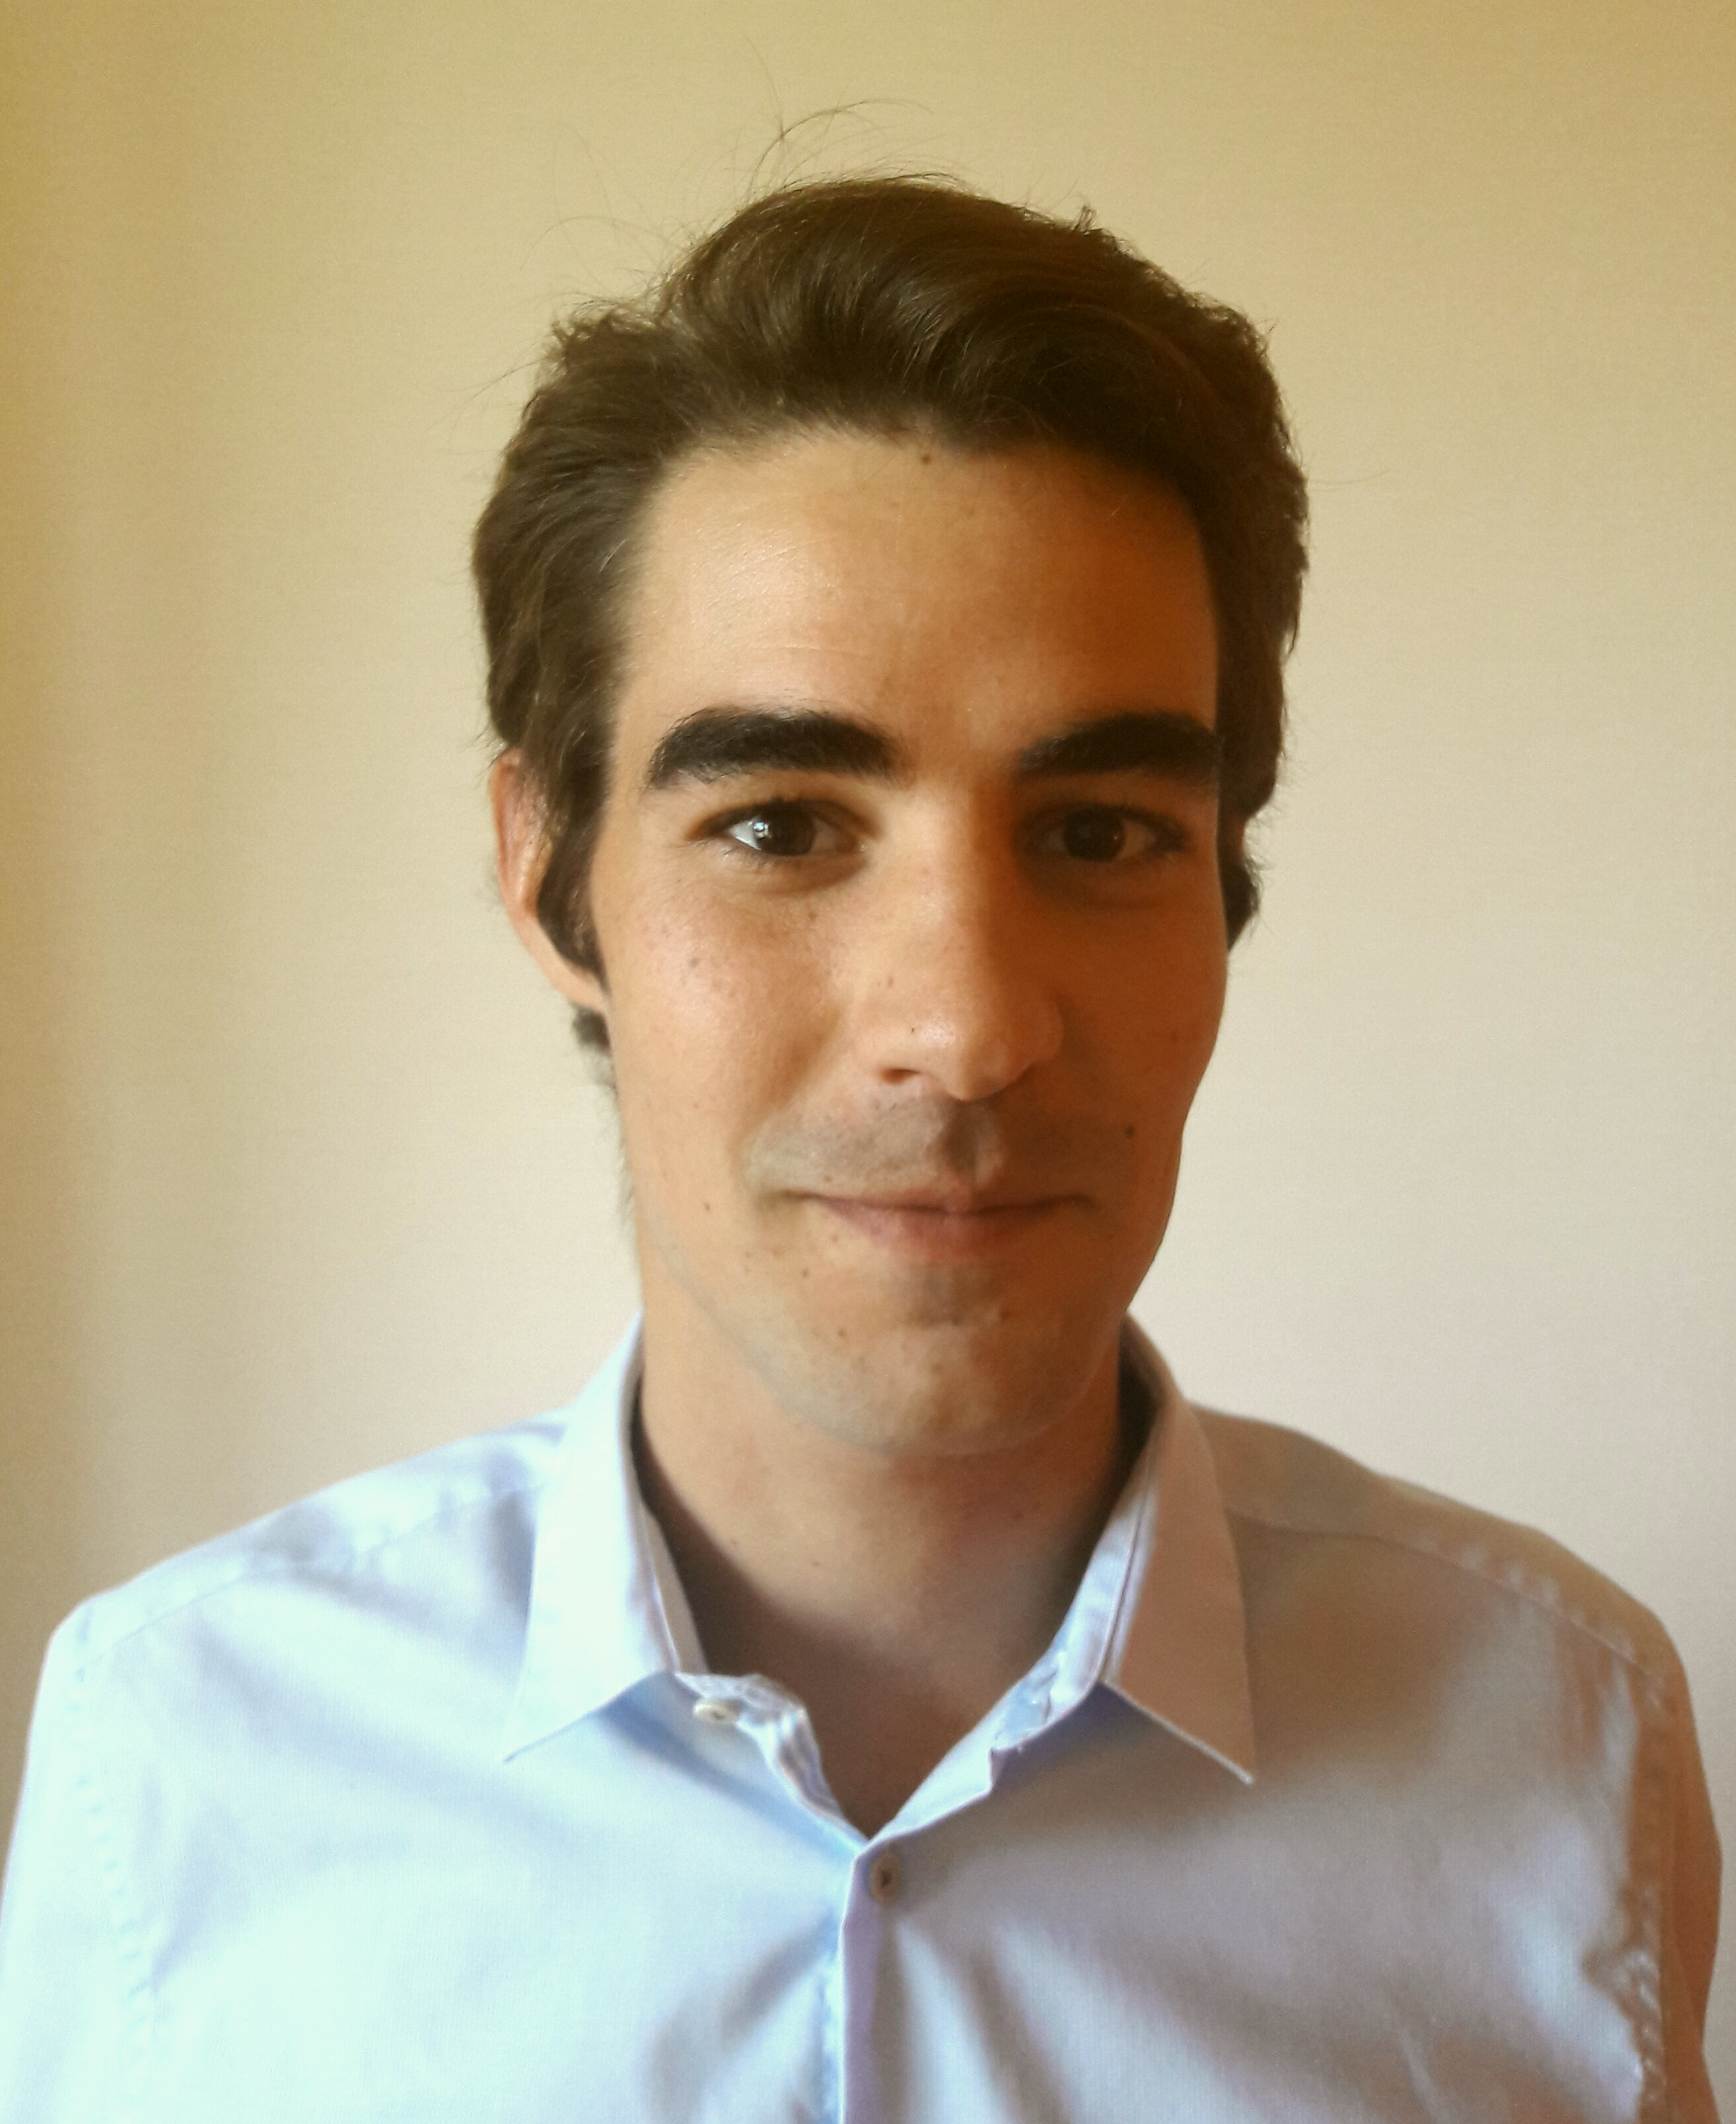
\includegraphics[height=75pt]{photo.png}
  \hfill\vfill
\end{wrapfigure}

~\
\makecvtitle % Print the CV title e

\vspace{-0.7cm}

{{\bfseries{Keywords}}: materials, nanosciences, optoelectronics, modelisation, optimization}

%----------------------------------------------------------------------------------------
%	DOCTORAT
%----------------------------------------------------------------------------------------
~\
\section{Doctoral Thesis}
\vspace{0.2cm}

\cvitem{2012--2015}{\emph{\bfseries \underline{Title}: Study of Semiconductor Nanoparticules Properties for Hybrid Solar Cells}}
\cvitem{Description}{\textbf{Governmental Grant with Teaching Position} at the Materials, Microelectronics and Nanosciences Institute of Provence (IM2NP - \textsc{Marseille}, France) within the Optoelectronics and Photovoltaics (OPTOPV) Team. Key points of this work include:
\begin{itemize}
\item Calculations of the physical properties of quantum structures
\item Experimental characterizations of nanoparticles incorporated in thin-films
\item Participation on various computational optoelectronics related works
\end{itemize}
}

%----------------------------------------------------------------------------------------
%	EXPERIENCES PROFESSIONNELLES
%----------------------------------------------------------------------------------------

\section{Work Experience}
\vspace{0.2cm}


\subsection{Research Internship - 6 months}
\cventry{January 2013 July 2013}{\textsc{Leopold-Franzens University}}{\textsc{Innsbr\"uck} (Austria)}{photonics team}{}{\textbf{Study of the foundations of quantum mechanics with single photon sources}
\begin{itemize}
\item Test of Born's law with three then five slits quantum experiments
\item Use of two sources: manufacture of an optical heralded single-photon source (with a non-linear cristal) and use of the emission from an isolated quantum dot
\end{itemize}
}
~\
\newline{}

\subsection{R$\&$D Internship - 6 months}
\cventry{August 2010 Feb. 2011}{\textsc{Fraunhofer IPM}}{\textsc{Kaiserslautern} (Germany)}{therahertz measurement and systems team}{}{\textbf{Characterization and optimization of a novel all electronic terahertz system}
\begin{itemize}
\item Use and optimization of the new non-destructive THz imaging system
\item Development of an hyperspectral image processing software (Matlab)
\end{itemize}
}
~\
\newline{}

\subsection{R$\&$D Internship - 3 months}
\cventry{April 2009 July 2009}{\textsc{LERM}}{\textsc{Arles} (France)}{materials study and research laboratory}{}{\textbf{Study of durability indicators in concrete and implementation of a new test method based on water permeability}
\begin{itemize}
\item Characterizations and durability studies of numerous samples
\item Use and characterization of the new test method
\end{itemize}
}

~\
\newline{}
%----------------------------------------------------------------------------------------
%	EDUCATION SECTION
%----------------------------------------------------------------------------------------
\section{Education}
\vspace{0.2cm}

% \cventry{2003--2006}{Ing�nieur G�nie Physique}{Polytech' Clermont-Ferrand (Ex. CUST)}{\textsc{Clermont-Ferrand}}{}{Sp�cialisation en Science des Mat�riaux}  % Arguments not required can be left empty
\cventry{2011--2012}{Master of Sciences}{in Mechanics and Physics with a specialty in Optics and Nanotechnologies (ONT)}{\textsc{University of Technology of Troyes (UTT)}}{}{}
\cventry{2009--2012}{Master of Engineering}{in Materials, Technology and Economy (MTE) with a speciality in Transformation and Quality of Materials (TQM)}{\textsc{University of Technology of Troyes (UTT)}}{}{}
\cventry{2007--2009}{DUT (technical degree)}{in Materials Science}{\textsc{Fran\c{c}ois Rabelais University}}{\newline{}IUT of Blois}{}

~\
\vspace{-0.2cm}
%----------------------------------------------------------------------------------------
%	COMMUNICATION SKILLS SECTION
%----------------------------------------------------------------------------------------
\section{Publications}

\cvitem{}{
Articles are available to download on \href{https://www.researchgate.net/profile/Francois_Thierry}{\bfseries ResearchGate} and \href{https://github.com/Francois-Thierry/about-me/tree/master/publications}{\bfseries GitHub}
}

\vspace{0.3cm}
%
\cvitem{2016}{ -
J. Le Rouzo, D. Duch\'e, C. Ruiz-Herrero, {\bfseries F. Thierry}, M. Carlberg, G. Berginc, M. Pasquinelli, J-J. Simon, L. Escoubas, and F. Flory,
"Specific tools for studying the optical response of heterogeneous thin film layers", Journal of Nanophotonics - submitted
}
\cvitem{}{ -
J. Le Rouzo, D. Duch\'e, C.M. Ruiz, {\bfseries F. Thierry}, M. Carlberg, G. Berginc, M. Pasquinelli, J.J. Simon, L. Escoubas and F. Flory,
"Characterization and modeling tools for light management in heterogeneous thin film layers", Proceedings of SPIE - The International Society for Optical Engineering 99290I \href{http://dx.doi.org/10.1117/12.2237682}{[link]}
}
\cvitem{2015}{ -
{\bfseries F. Thierry}, J. Le Rouzo, F. Flory, G. Berginc and L. Escoubas,
"Fast and reliable approach to calculate energy levels in semiconductor nanostructures", Journal of Nanophotonics, 9(1), 093080. \href{http://dx.doi.org/10.1117/1.JNP.9.093080}{[link]}
}
\cvitem{2014}{ -
A. Bou, P. Torchio, D. Barakel, {\bfseries F. Thierry}, A. Sangar, P-Y. Thoulon and M. Ricci, "Indium tin oxide-free transparent and conductive electrode based on SnOx | Ag | SnOx for organic solar cells", Journal of Applied Physics, 116, 023105 \href{http://dx.doi.org/10.1063/1.4886225}{[link]}
}
\cvitem{}{ -
{\bfseries F. Thierry}, J. Le Rouzo, F. Flory, G. Berginc and L. Escoubas, "Optimization of the optical properties of nanostructures through fast numerical approaches", Proceedings of SPIE - The International Society for Optical Engineering 916102 \href{http://dx.doi.org/10.1117/12.2061042}{[link]}
}
\cvitem{}{ -
A. Bou, P. Torchio, D. Barakel, {\bfseries F. Thierry}, P-Y. Thoulon and M. Ricci,  "Numerical and experimental study of SnOx | Ag | SnOx multilayer as indium-free transparent electrode for organic solar cells", Proceedings of SPIE - The International Society for Optical Engineering 898706 \href{http://dx.doi.org/10.1117/12.2039067}{[link]}
}

~\
\vspace{0.3cm}
%----------------------------------------------------------------------------------------
%	AWARDS SECTION
%----------------------------------------------------------------------------------------
\section{Awards and Distinctions}
\vspace{0.2cm}

\cvitem{2014}{ - Newport Research Excellence Award - SPIE Optics + Photonics, San Diego, USA}
\cvitem{}{ - Best Poster Award - Journ\'ees de l'IM2NP, Cassis, France}

%----------------------------------------------------------------------------------------
%	COMPUTER SKILLS SECTION
%----------------------------------------------------------------------------------------
~\
\section{Computer Skills}
\vspace{0.2cm}

\cvitem{Programming}{{\bfseries Python}, C/C++, HTML/Javascript, Matlab}
\cvitem{Office Soft.}{{\bfseries \LaTeX}, Microsoft Office, Reveal.js}
\cvitem{Graph./CAO}{{\bfseries Inkscape}, Gimp, Photoshop / Autodesk Inventor}


%----------------------------------------------------------------------------------------
%	LANGUAGES SECTION
%----------------------------------------------------------------------------------------
~\
\section{Languages}
\vspace{0.2cm}

\cvitem{French}{Mother tongue}{}
\cvitem{{\bfseries English}}{Fluent}{}
\cvitem{{\bfseries German}}{Fluent}{}
\cvitem{Espagnol}{Notions}{}
\cvitem{Italian}{Notions}{}

%----------------------------------------------------------------------------------------

\end{document}